\documentclass{article}

\usepackage{graphicx}
\usepackage{tikz}
\usepackage{tikzsymbols}
\usetikzlibrary{calc,patterns,shapes.geometric}
\pagestyle{empty}
\usepackage[margin=0pt]{geometry}
\geometry{papersize={14in,12in}}

\def\centerarc[#1](#2)(#3:#4:#5){\draw[#1] ($(#2)+({#5*cos(#3)},{#5*sin(#3)})$) arc (#3:#4:#5);}

\begin{document}
	\begin{figure}
		\centering
		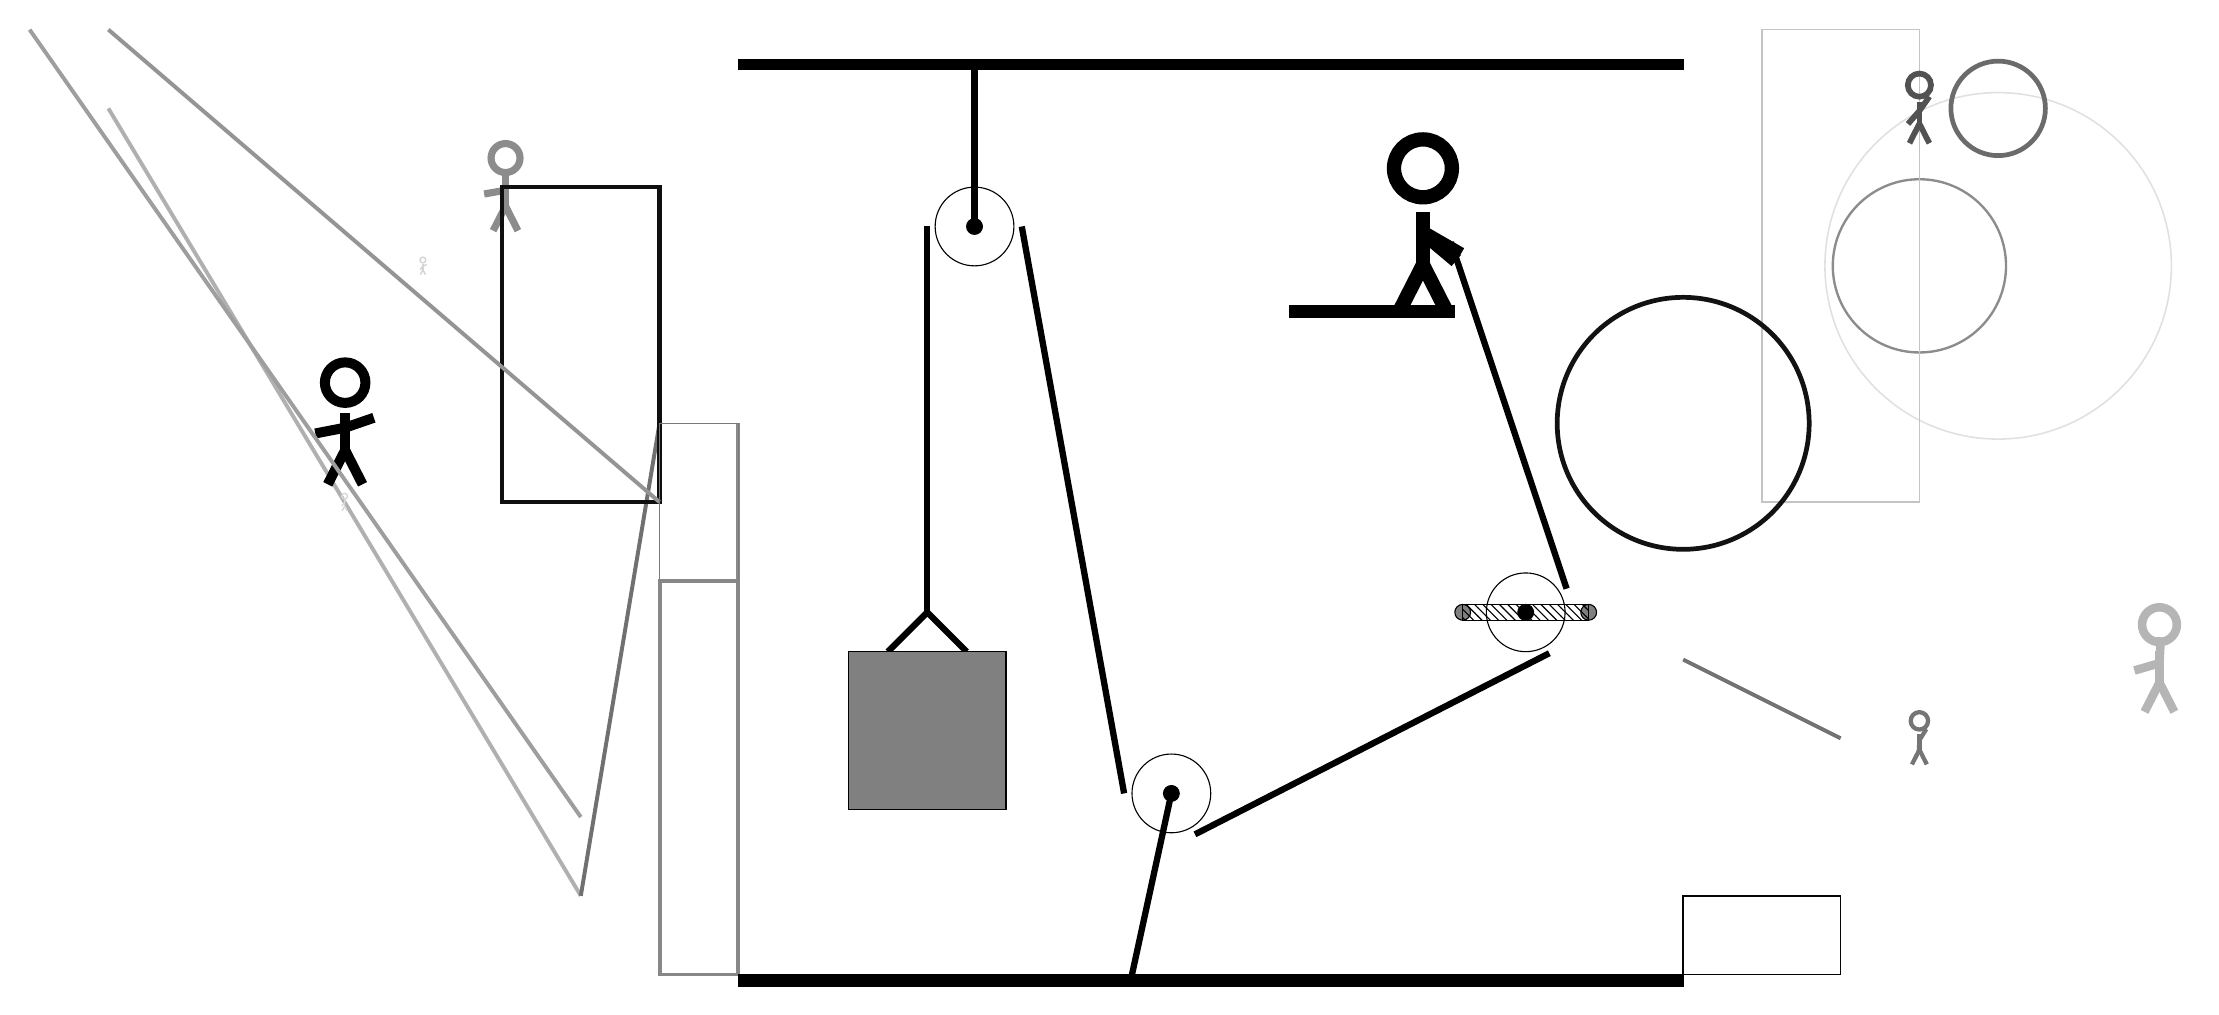
\begin{tikzpicture}
			%%%%% START %%%%%
			
			\draw[fill=black] (-2, 11.5) rectangle (10, 11.625);
			
			\draw (1, 9.5) circle (0.5);
			\draw[fill=black] (1, 9.5) circle (0.1);
			\draw[line width=0.8mm] (1, 11.5) -- (1, 9.5);
			
			\draw (3.5, 2.3) circle (0.5);
			\draw[fill=black] (3.5, 2.3) circle (0.1);
			\draw[line width=0.8mm] (3.5, 2.3) -- (3.0, 0);
			
			\draw[fill=white](8, 4.6) circle (0.5);
			\draw[fill=black] (8, 4.6) circle (0.1);
			\draw[fill=black!50] (8.8, 4.6) circle (0.1);
			\draw[fill=black!50] (7.2, 4.6) circle (0.1);
			\draw[pattern=north west lines, pattern color=black] (7.2, 4.7) rectangle (8.8, 4.5);
			
			\draw[line width=0.8mm](-0.1, 4.1) --  (0.4, 4.6) -- (0.9, 4.1);
			\draw[fill=black!50] (-0.6, 4.1) rectangle (1.4, 2.1);
			
			\draw[line width=0.8mm](0.4, 9.5) -- (0.4, 4.6);
			\centerarc[line width=0.8mm](1, 9.5)(180:0:0.6)
			\draw[line width=0.8mm](1.6, 9.5) -- (2.9, 2.3);
			\centerarc[line width=0.8mm](3.5, 2.3)(180:300:0.6);
			\draw[line width=0.8mm](3.8, 1.7804) -- (8.3, 4.0804);
			\centerarc[line width=0.8mm](8, 4.6)(300:390:0.6);
			\draw[line width=0.8mm](8.5196, 4.9) -- (7.05, 9.3);
			
			\node at (6.75, 9.5) {\Strichmaxerl[10][-220][-30]};
			\draw[fill=black] (5, 8.5) rectangle (7.1, 8.35);
			
			\draw[line width=0.5mm, color=black!31](-4, 1) -- (-10, 11);
			
			\draw[line width=0.2mm, color=black!98] (12, 1) rectangle (10, 0);
			\node[line width=0.2mm, color=black!17] at (-6, 9) {\Strichmaxerl[1][47][28]};
			\draw[line width=0.5mm, color=black!46](-2, 4) -- (-2, 7);
			\draw [line width=0.3mm, color=black!45](13, 9) circle (1.1);
			\node[line width=0.6mm, color=black!45] at (-5, 10) {\Strichmaxerl[5][10][90]};
			\draw [line width=0.2mm, color=black!12](14, 9) circle (2.2);
			\node[line width=0.6mm, color=black!54] at (13, 3) {\Strichmaxerl[3][87][58]};
			\draw[line width=0.5mm, color=black!56](-3, 7) -- (-4, 1);
			\node[line width=0.3mm, color=black!100] at (-7, 7) {\Strichmaxerl[7][11][19]};
			
			\draw[line width=0.2mm, color=black!23] (11, 12) rectangle (13, 6);
			\draw[line width=0.6mm, color=black!94] (-3, 6) rectangle (-5, 10);
			\draw[line width=0.5mm, color=black!42](-3, 6) -- (-10, 12);
			
			\node[line width=0.6mm, color=black!68] at (13, 11) {\Strichmaxerl[4][49][55]};
			\draw [line width=0.6mm, color=black!58](14, 11) circle (0.6);
			\draw[line width=0.5mm, color=black!38](-4, 2) -- (-11, 12);
			\draw[line width=0.2mm, color=black!52] (-2, 0) rectangle (-3, 7);
			
			\node[line width=0.4mm, color=black!29] at (16, 4) {\Strichmaxerl[6][16][87]};
			\node[line width=0.4mm, color=black!15] at (-7, 6) {\Strichmaxerl[1][46][77]};
			\draw [line width=0.6mm, color=black!93](10, 7) circle (1.6);
			\draw[line width=0.5mm, color=black!47] (-2, 5) rectangle (-3, 0);
			
			\draw[line width=0.5mm, color=black!55](10, 4) -- (12, 3);
			
			\draw[fill=black] (-2, 0) rectangle (10, -0.15);
			
			%%%%% END %%%%%
		\end{tikzpicture}
	\end{figure}	
\end{document}